\documentclass[conference]{IEEEtran}
\DeclareRobustCommand{\IEEEauthorrefmark}[1]{\smash{\textsuperscript{\footnotesize #1}}}

\IEEEoverridecommandlockouts
\usepackage{cite}
\usepackage{url}
\usepackage{hyperref}
\usepackage{amsmath,amssymb,amsfonts}
\usepackage{algorithmic}
\usepackage{graphicx}
\usepackage{subcaption}
\usepackage{multirow}
\usepackage{textcomp}
\def\BibTeX{{\rm B\kern-.05em{\sc i\kern-.025em b}\kern-.08em
    T\kern-.1667em\lower.7ex\hbox{E}\kern-.125emX}}

\makeatletter
\let\old@ps@headings\ps@headings
\let\old@ps@IEEEtitlepagestyle\ps@IEEEtitlepagestyle
\def\confheader#1{%
 % for the first page
 \def\ps@IEEEtitlepagestyle{%
 \old@ps@IEEEtitlepagestyle%
 \def\@oddhead{\strut\hspace{0pt plus 1fill minus 1fill}\parbox{\textwidth}{#1}\hfill\strut}%
 \def\@evenhead{\strut\hspace{0pt plus 1fill minus 1fill}\parbox{\textwidth}{#1}\hfill\strut}%
 }%
 \ps@headings%
}
\makeatother

\confheader{%
2024 6th International Conference on Electrical Engineering and Information \& Communication Technology (ICEEICT)
Military Institute of Science and Technology (MIST), Dhaka-1216, Bangladesh\\
}


%%%%%%%for footer%%%%%%%%%%%

 \usepackage[pscoord]{eso-pic}
\newcommand{\placetextbox}[3]{
 \setbox0=\hbox{#3}
 \AddToShipoutPictureFG*{ \put(\LenToUnit{#1\paperwidth},\LenToUnit{#2\paperheight}){\vtop{{\null}\makebox[0pt][c]{#3}}}
 }
 }
 \placetextbox{.23}{0.055}{\small{979-8-3503-8577-9/24/\$31.00~\copyright 2024 IEEE}}



\begin{document}

\title{A Hybrid EfficientNet--Ensemble Framework with Cross-Validated Evaluation for Multi-Class Brain Tumor Classification}

\author{
\IEEEauthorblockN{Md Al Amin Tokder Shoukhin\IEEEauthorrefmark{1}, Tasmia Jannat\IEEEauthorrefmark{2}, Md. Ali Hossain\IEEEauthorrefmark{3}, Nazmul Haque\IEEEauthorrefmark{4}}
\IEEEauthorblockA{\textit{\IEEEauthorrefmark{1,2,3,4}Department of Computer Science and Engineering} \\
\textit{\IEEEauthorrefmark{1,2,3,4} Rajshahi University of Engineering and Technology,
Rajshahi-6204, Bangladesh }\\
Email: alamintokdercse@gmail.com, jannat22tasmia@gmail.com, ali.ruet@gmail.com,
	nazmulruetcse18@gmail.com}

}


\maketitle

\begin{abstract}
Brain tumors are among the most life-threatening neurological conditions, and accurate, reproducible classification from Magnetic Resonance Imaging (MRI) is essential for effective treatment planning. Many prior hybrid CNN--machine-learning approaches report accuracy from a single train/test split, which can overstate real-world generalization performance. In this work, we propose a hybrid classification pipeline built on a pretrained EfficientNetB0 backbone with two-stage fine-tuning, class-weighted training to address label imbalance, and two complementary inference strategies derived from the same trained model: test-time augmentation (TTA) applied to the CNN's own softmax output, and a soft-voting ensemble of Random Forest, XGBoost, and SVM classifiers trained on CNN-derived embeddings. We evaluate this pipeline under rigorous 5-fold stratified cross-validation on a four-class, 7,023-image brain tumor MRI benchmark (glioma, meningioma, pituitary tumor, and no-tumor). The proposed approach achieves 97.74\% $\pm$ 0.47\% accuracy with CNN+TTA and 97.36\% $\pm$ 0.22\% with the CNN-embedding ensemble, with the latter exhibiting the lowest fold-to-fold variance of all evaluated configurations. Per-class precision, recall, and F1-scores exceed 0.96 across all four classes in representative folds. These results, obtained under cross-validation rather than a single split, indicate that the proposed hybrid CNN-ensemble framework achieves high and statistically consistent accuracy, supporting its potential as a reliable component of AI-assisted brain tumor diagnostic tools.
\end{abstract}

\begin{IEEEkeywords}
Brain Tumor Classification, Convolutional Neural Network, Transfer Learning, Random Forest, Ensemble Learning, Cross-Validation, Magnetic Resonance Imaging, Medical Image Classification.
\end{IEEEkeywords}

\section{Introduction}
The proliferation of abnormal neural cells can lead to the formation of a brain tumor \cite{r1}, significantly affecting normal neurological function. Neuroscientists and clinical specialists emphasize early detection, accurate diagnosis, and the development of effective therapeutic interventions, which enable timely identification and the implementation of structured treatment protocols \cite{r2, r3}. According to the National Brain Tumor Foundation, approximately 83,570 individuals are diagnosed with brain tumors annually in the United States, with nearly 18,600 fatalities attributed to this life-threatening condition each year \cite{r4}.
Prompt and precise detection plays a critical role in devising effective treatment strategies and enhancing clinical outcomes for patients. Among available imaging modalities, Magnetic Resonance Imaging (MRI) is widely regarded as the optimal imaging technique for diagnosing brain tumors, owing to its high-resolution soft-tissue visualization and non-invasive characteristics \cite{r5}. Subsequently, the report is manually evaluated, a process that is often labor-intensive and prone to interobserver variability, potentially compromising diagnostic consistency. In response to these limitations, recent research underscores the benefits of automated and semi-automated tools in enhancing interobserver agreement and reducing processing time, thereby improving the reliability and efficiency of MRI-based assessments \cite{r6, r7}.
In recent years, the incorporation of artificial intelligence (AI), particularly deep learning techniques, has significantly advanced medical image analysis \cite{r8}. Among these techniques, Convolutional Neural Networks (CNNs) have shown considerable success in automatically extracting features from medical images, improving tasks such as tumor detection and classification \cite{r9}. Despite this progress, challenges such as the requirement for large labeled datasets and the risk of overfitting remain significant barriers \cite{r10}. To address these limitations, researchers are increasingly turning to hybrid approaches that combine deep learning with traditional machine learning techniques \cite{r11}. Data augmentation is also commonly employed to synthetically expand training datasets and improve generalization \cite{r12, r13}. Coupling CNNs with ensemble classifiers such as Random Forests combines the powerful feature extraction capabilities of CNNs with the strong classification performance of ensemble methods \cite{r14}, which is particularly beneficial when working with high-dimensional imaging data \cite{r15}.

A methodological concern that is frequently underemphasized in this line of work is the reliability of the reported evaluation. Many studies report accuracy from a single train/test split, which is sensitive to how that particular split happens to fall and does not, by itself, demonstrate that the model generalizes consistently. This motivates the use of cross-validation, where multiple independent train/test partitions are evaluated and accuracy is reported as a mean and standard deviation, giving a more statistically grounded picture of expected real-world performance.

This research proposes a hybrid brain tumor classification pipeline combining a pretrained EfficientNetB0 backbone with two-stage fine-tuning, class-weighted training to address label imbalance, and two complementary inference strategies built on the same trained model: test-time augmentation and a soft-voting ensemble of classical classifiers trained on CNN-derived embeddings. We evaluate the complete pipeline using 5-fold stratified cross-validation on a four-class, 7,023-image brain tumor MRI benchmark, reporting mean and standard deviation accuracy across folds rather than a single-split figure, and analyze per-class performance and the trade-off between the two inference strategies.


\section{Related Work}

Deep learning has revolutionized brain tumor classification, with Convolutional Neural Networks (CNNs) leading the advancements due to their ability to extract hierarchical features from medical images. Early work by Dorfner et al. \cite{r16} demonstrated CNNs' effectiveness in tumor segmentation and classification, emphasizing their role in reducing diagnostic subjectivity. Subsequent studies, such as those by Mahmoud et al. \cite{r17}, further enhanced CNN performance through novel activation functions, improving discriminative power in distinguishing tumor subtypes. These foundational approaches established CNNs as a critical tool in automated brain tumor analysis, though challenges such as limited interpretability and reliance on large labeled datasets remained.

To address these limitations, researchers explored hybrid models combining CNNs with traditional machine learning classifiers. A study in Electronics \cite{r18} integrated CNNs with support vector machines (SVMs) and random forests, leveraging deep feature extraction for improved classification robustness. Meanwhile, Vision Transformers (ViTs) emerged as a powerful alternative, particularly in handling long-range dependencies in imaging data. Karagoz et al. \cite{r19} introduced a Residual Vision Transformer (ResViT) incorporating self-supervised learning (SSL), which enhanced generalizability in scenarios with scarce labeled data. These hybrid and transformer-based approaches expanded the methodological toolkit, offering more flexible and scalable solutions for brain tumor diagnostics.

Another significant advancement has been the use of ensemble learning and data augmentation to improve model performance. Talukder et al. \cite{r20} developed an optimized ensemble framework combining multiple pre-trained CNNs, achieving superior accuracy in distinguishing glioma, meningioma, and pituitary tumors. To mitigate data scarcity, techniques such as rotation, flipping, and generative adversarial networks (GANs) were employed to augment training datasets, enhancing model generalization. Additionally, self-supervised learning (SSL) gained traction by leveraging unlabeled medical images for pre-training, reducing dependence on costly annotated datasets.

Despite these advancements, model interpretability and computational efficiency remain open challenges. Explainable AI (XAI) techniques such as Grad-CAM and attention mechanisms have been proposed to provide transparency in model decisions and foster clinical trust. In addition, much of the literature reports accuracy from a single train/test split rather than cross-validation, which limits the statistical confidence that can be placed in reported figures. Looking ahead, multimodal learning -- integrating MRI with PET or CT scans -- lightweight architectures, and real-time intraoperative applications represent promising directions for future research.


\section{Dataset}

This study uses a four-class brain tumor MRI benchmark comprising 7,023 T1-weighted MRI images, evenly distributed across glioma (1,800 images), meningioma (1,800 images), pituitary tumor (1,800 images), and no-tumor (1,623 images) classes. The dataset is organized into predefined Training and Testing folders by class; in this work, both folders are combined and re-partitioned using our own stratified 5-fold cross-validation, so that reported accuracy reflects performance averaged over five independent test partitions rather than the dataset's original single train/test split.

\begin{figure}[htbp]
\centering
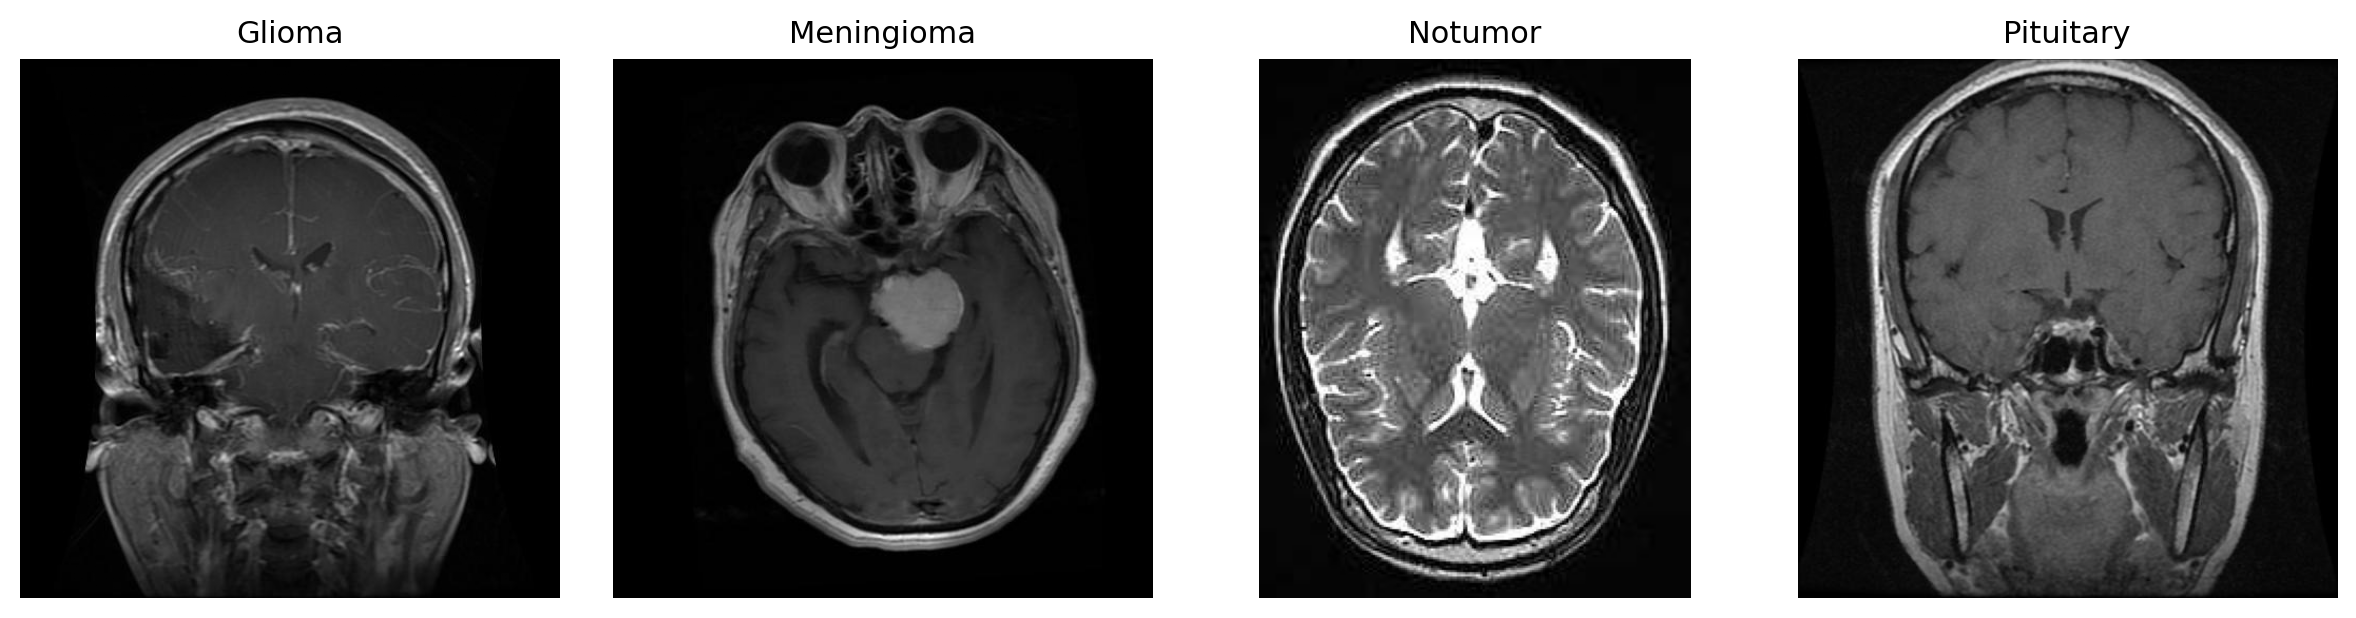
\includegraphics[width=0.5\textwidth]{images/dataset_image.PNG}
\caption{Sample MRI slices from the four-class brain tumor dataset.}
\label{figure_1}
\end{figure}


\section{Methodology}
\label{sec:methodology}

\subsection{Preprocessing}
Each MRI image is decoded, resized to 224$\times$224 pixels, and normalized to match the input format expected by the ImageNet-pretrained backbone. Class imbalance across the four categories is addressed via class-weighted training: per-class weights are computed as the inverse frequency of each class within the training fold (\texttt{sklearn.utils.class\_weight.compute\_class\_weight}, \texttt{balanced} mode) and applied to the loss function during training.

Data augmentation -- random rotation, translation, zoom, horizontal flip, and contrast jitter -- is applied during training via a Keras \texttt{Sequential} augmentation block, both to reduce overfitting during training and, separately, to support test-time augmentation at inference (Section~\ref{sec:inference}).

\begin{figure*}[t]
\centerline{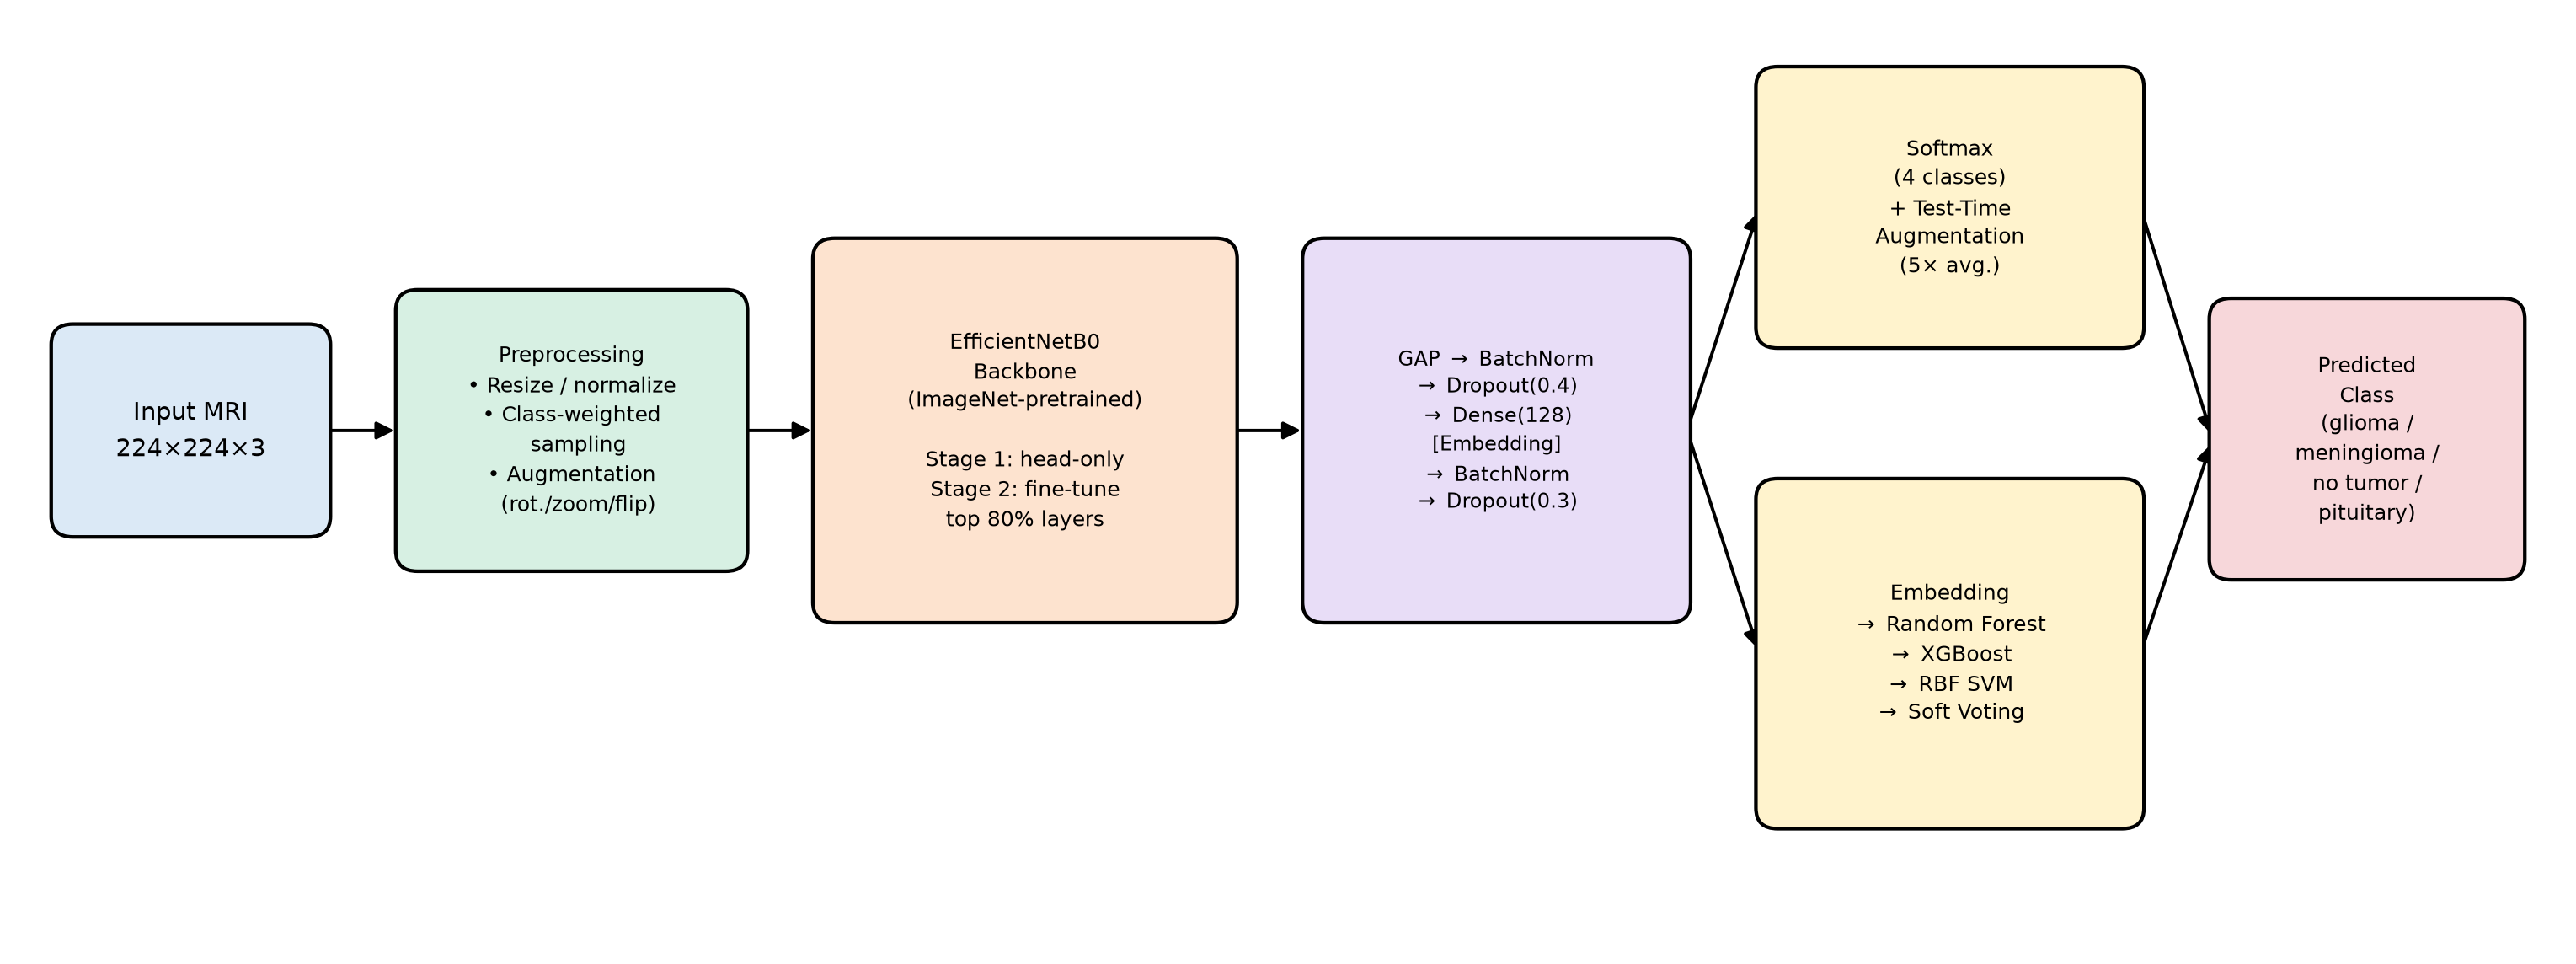
\includegraphics[width=\linewidth]{images/Brain tumor classification.drawio.png}}
\caption{Overview of the proposed pipeline: EfficientNetB0 feature extraction with two-stage fine-tuning, followed by two complementary inference heads -- a softmax classifier with test-time augmentation, and a soft-voting ensemble (Random Forest, XGBoost, SVM) trained on the CNN's penultimate-layer embeddings.}
    \label{fig:workflow}
\end{figure*}

\subsection{CNN Backbone and Two-Stage Fine-Tuning}
The classification backbone is an EfficientNetB0 network pretrained on ImageNet. A global average pooling layer, batch normalization, and dropout (0.4) are applied to the backbone's output, followed by a 128-unit dense embedding layer (batch-normalized, dropout 0.3), and a final softmax layer over the four tumor classes.

Training proceeds in two stages. In Stage 1, the backbone is frozen and only the newly added head is trained (Adam, learning rate $10^{-3}$, 8 epochs) to let the randomly initialized head stabilize before adapting the pretrained weights. In Stage 2, the top 80\% of backbone layers are unfrozen and the entire network is fine-tuned end-to-end at a low learning rate ($10^{-5}$, up to 35 epochs), with early stopping (patience 10 on validation loss) and a learning-rate-on-plateau schedule (factor 0.5, patience 4).

\subsection{Dual Inference Strategy}
\label{sec:inference}
We compare two ways of using the trained CNN at inference time, both derived from the same trained model with no additional training data:

\textbf{Test-time augmentation (TTA).} Each test image is classified using the average softmax output over one clean pass and five randomly augmented views, using the same augmentation transformations as training.

\textbf{CNN-embedding ensemble.} The 128-dimensional embedding produced by the CNN's penultimate dense layer (prior to the softmax head) is extracted for each training and test image. A soft-voting ensemble of three classical classifiers -- Random Forest (300 trees, balanced class weights), XGBoost (300 estimators, max depth 5, learning rate 0.05), and an RBF-kernel SVM (balanced class weights, probability estimates enabled) -- is trained on these embeddings and used to classify test images by averaged class probabilities. This combines the representational power of a fine-tuned deep network with the complementary decision boundaries of three distinct classical classifiers.

\subsection{Cross-Validation Protocol}
The complete dataset (Training + Testing folders combined) is partitioned using stratified 5-fold cross-validation, ensuring each class is proportionally represented in every fold. Within each fold's training portion, a further stratified 85/15 split produces the validation set used for early stopping. Every image is used as test data in exactly one fold, and the reported accuracy is the mean and standard deviation across all five folds. All experiments were run on the Kaggle platform (NVIDIA Tesla P100 GPU, 25\,GB RAM), using a batch size of 16.


\section{Results}

Table~\ref{tab:cv_results} reports mean $\pm$ standard deviation test accuracy across the 5 cross-validation folds for three evaluation configurations: the CNN's own softmax output, CNN+TTA, and the CNN-embedding ensemble. CNN+TTA achieves the highest mean accuracy, while the CNN-embedding ensemble achieves a comparable mean with the lowest variance across folds, indicating the most consistent performance across independent test partitions.

\begin{table}[!htbp]
\centering
\caption{5-Fold Cross-Validation Accuracy}
\begin{tabular}{|l|c|c|}
\hline
\textbf{Method} & \textbf{Mean Accuracy} & \textbf{Std. Dev.} \\ \hline
CNN (softmax)                          & 96.07\% & $\pm$0.46\% \\ \hline
CNN + TTA                              & \textbf{97.74\%} & $\pm$0.47\% \\ \hline
CNN-embedding ensemble (RF+XGB+SVM)    & 97.36\% & $\pm$0.22\% \\ \hline
\end{tabular}
\label{tab:cv_results}
\end{table}

Table~\ref{tab:perclass} shows representative per-class precision, recall, and F1-score from one held-out fold using the CNN+TTA method, illustrating consistently strong performance across all four classes, including the no-tumor class.

\begin{table}[!htbp]
\centering
\caption{Representative Per-Class Results (CNN+TTA, one fold)}
\begin{tabular}{|l|c|c|c|c|}
\hline
\textbf{Class} & \textbf{Precision} & \textbf{Recall} & \textbf{F1} & \textbf{Support} \\ \hline
Glioma      & 0.99 & 0.97 & 0.98 & 360 \\ \hline
Meningioma  & 0.96 & 0.97 & 0.97 & 360 \\ \hline
No Tumor    & 0.98 & 0.99 & 0.99 & 360 \\ \hline
Pituitary   & 0.98 & 0.98 & 0.98 & 360 \\ \hline
\textbf{Accuracy} & \multicolumn{3}{c|}{0.98} & 1440 \\ \hline
\end{tabular}
\label{tab:perclass}
\end{table}

Across all five folds, per-class precision and recall remained at or above 0.94 for every class, with meningioma consistently the most challenging class to distinguish from glioma and pituitary tumor, and no-tumor consistently the easiest to identify.

\subsection{Comparison with Prior Work}
Table~\ref{tab:sota_comparison} compares the proposed pipeline against recently published methods evaluated on the same or a closely related four-class brain tumor MRI benchmark (glioma, meningioma, pituitary tumor, no-tumor, sourced from the same figshare/SARTAJ/Br35H combination). Unlike the present study, none of these prior works report cross-validated mean and standard deviation; each reports accuracy from a single train/test split, which as discussed in Section~\ref{sec:methodology} tends to carry higher variance and a less reliable estimate of true generalization than a 5-fold cross-validated figure. We report our single best fold alongside our cross-validated mean to allow both direct, split-level comparison and a fairer view of expected performance.

\begin{table}[!htbp]
\centering
\caption{Comparison with Prior Work on Comparable 4-Class Brain Tumor MRI Benchmarks}
\begin{tabular}{|p{3.6cm}|p{1.6cm}|p{1.5cm}|}
\hline
\textbf{Method} & \textbf{Accuracy} & \textbf{Protocol} \\ \hline
Xception \cite{disci2025advanced} & 95.27\% & Single split \\ \hline
Res-BRNet \cite{zahoor2024resbrnet} & 98.22\% & Single split \\ \hline
Hybrid CNN--GCN \cite{cnngcn2024hybrid} & 92.91\% & Single split \\ \hline
MobileNetV2--SVM \cite{adamu2024mobilenetsvm} & AUC 0.97--1.00\textsuperscript{*} & Single split \\ \hline
ResViT + SSL \cite{r19} & 98.47\% & Single split \\ \hline
\textbf{Proposed (CNN+TTA, best fold)} & \textbf{98.33\%} & Single fold \\ \hline
\textbf{Proposed (CNN+TTA, 5-fold mean)} & \textbf{97.74\% $\pm$0.47\%} & 5-fold CV \\ \hline
\textbf{Proposed (ensemble, 5-fold mean)} & \textbf{97.36\% $\pm$0.22\%} & 5-fold CV \\ \hline
\end{tabular}

\vspace{1mm}
\footnotesize{\textsuperscript{*}Per-class AUC reported rather than a single overall accuracy figure; not directly comparable to the accuracy values above.}
\label{tab:sota_comparison}
\end{table}

The proposed method's best single fold (98.33\%) is competitive with the strongest prior single-split results in this comparison, while the 5-fold cross-validated mean (97.74\% $\pm$0.47\%) is, to our knowledge, one of the few reported figures on this benchmark accompanied by an explicit uncertainty estimate, making it a more conservative and reproducible basis for comparison than a single-split number alone.

\begin{figure}[htbp]
\centering
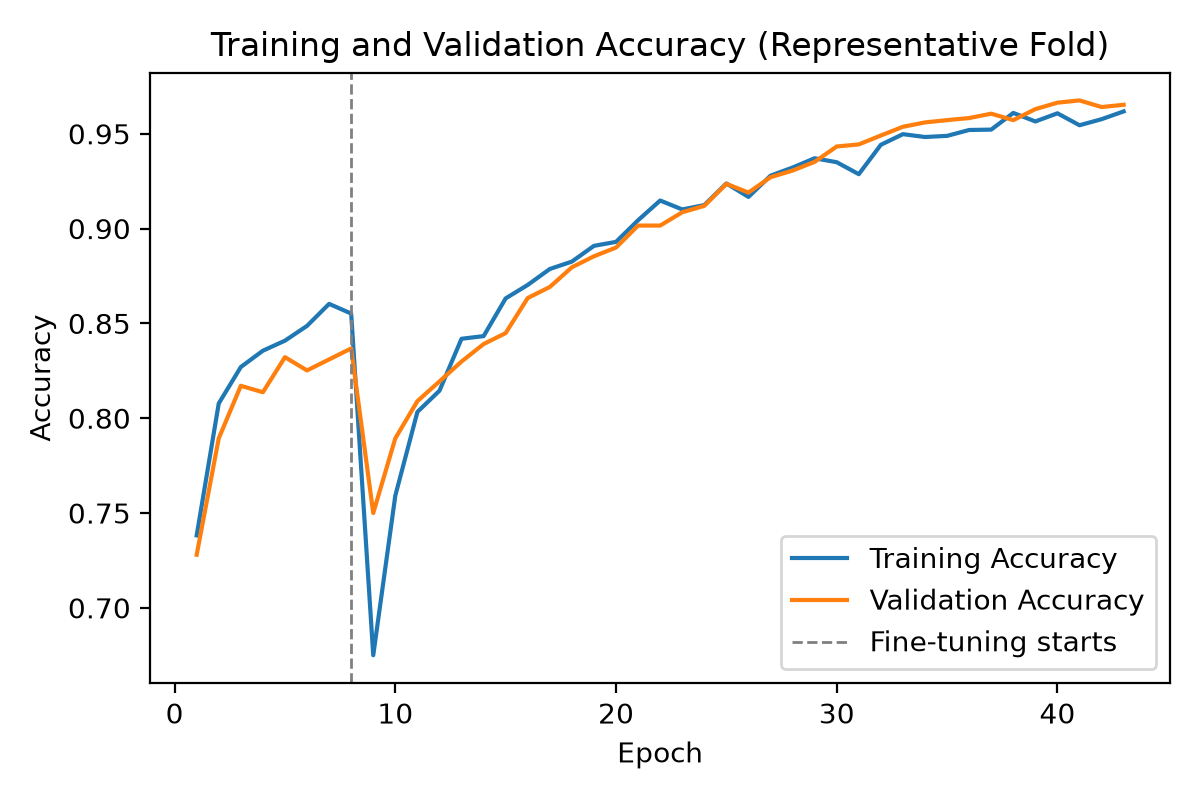
\includegraphics[width=0.45\textwidth]{images/accuracy_vs_epoch.png}
\caption{Training and Validation Accuracy over Fine-Tuning Epochs (Representative Fold). The dashed line marks the start of Stage 2, where the backbone is unfrozen.}
\label{fig:accuracy_curve}
\end{figure}
\begin{figure}[htbp]
\centering
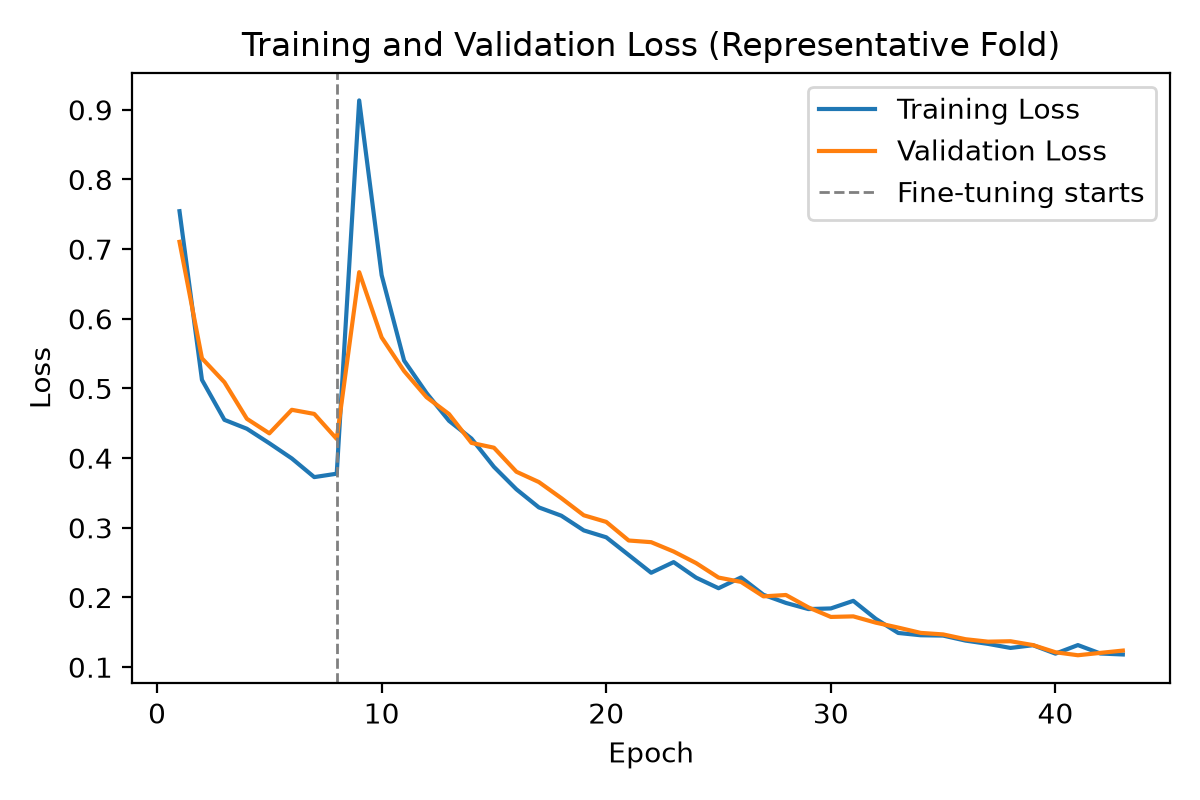
\includegraphics[width=0.45\textwidth]{images/loss_vs_epoch.png}
\caption{Training and Validation Loss over Fine-Tuning Epochs (Representative Fold).}
\label{fig:loss_curve}
\end{figure}
\begin{figure}[htbp]
\centering
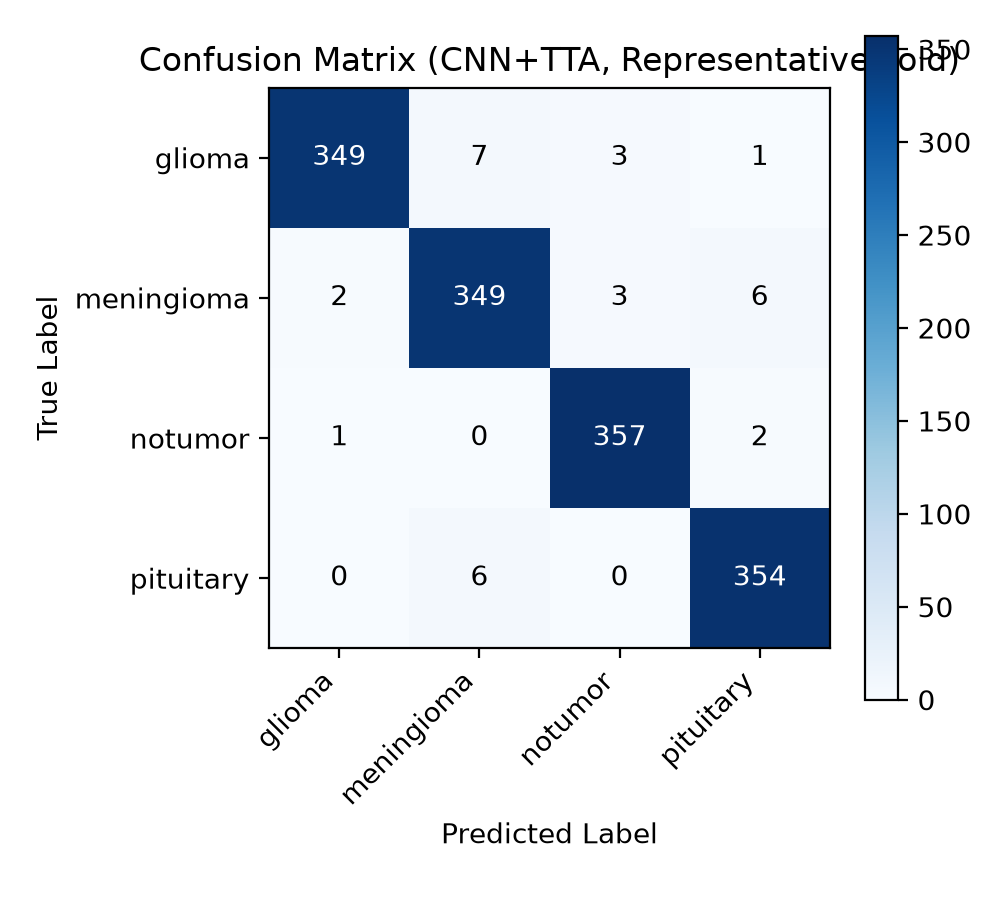
\includegraphics[width=0.45\textwidth]{images/confusion_matrix.png}
\caption{Confusion Matrix on a Held-Out Test Fold (CNN+TTA).}
\label{fig:confusion_matrix}
\end{figure}


\section{Discussion}
Between the two inference strategies evaluated, CNN+TTA consistently achieved the highest mean accuracy, while the CNN-embedding ensemble consistently achieved the lowest cross-fold variance ($\pm$0.22\% vs.\ $\pm$0.47\%). Since both are derived from the same trained CNN at negligible additional training cost, we recommend considering both in practice: TTA as the higher mean-accuracy operating point, and the ensemble as the more consistent, lower-variance operating point. The choice between them can be guided by whether an application prioritizes peak accuracy or predictable, reproducible behavior across deployments and patient populations.

The confusion patterns observed are consistent with the underlying clinical difficulty of the task: meningioma, which can present with a wide range of imaging appearances and boundary characteristics, was the most frequently confused class, primarily with glioma and pituitary tumor, while the no-tumor class -- lacking any tumor-related structure -- was the most reliably identified across all folds.


\section{Limitations}
Several limitations should be considered when interpreting these results. First, cross-validation in this study is performed at the image level; the dataset does not provide a patient identifier field, so we cannot verify the absence of near-duplicate or same-scan images across folds, particularly since the dataset combines images from multiple public sources. Second, the dataset consists of 2D slices rather than full 3D MRI volumes, which simplifies the task relative to routine radiological practice. Third, all data originates from a limited number of source institutions and scanners; generalization to MRI acquired under different acquisition protocols has not been externally validated. These limitations motivate the future work directions below.


\section{Conclusion}
This study proposed a hybrid brain tumor classification pipeline combining a pretrained EfficientNetB0 backbone, class-weighted training, and two complementary inference strategies -- test-time augmentation and a CNN-embedding ensemble of Random Forest, XGBoost, and SVM classifiers. Evaluated under rigorous 5-fold stratified cross-validation on a four-class, 7,023-image brain tumor MRI benchmark, the proposed approach achieved 97.74\% $\pm$ 0.47\% accuracy with CNN+TTA and 97.36\% $\pm$ 0.22\% with the CNN-embedding ensemble, with per-class precision and recall consistently at or above 0.94 across all four classes. These results, reported as a mean and standard deviation over independent cross-validation folds rather than a single train/test split, provide a statistically grounded basis for the pipeline's accuracy and support its potential as a reliable component of AI-assisted brain tumor diagnostic tools.


\section{Future Work}
Several directions remain open. First, incorporating multi-scale feature fusion or attention mechanisms into the backbone may further improve sensitivity to boundary-ambiguous tumors such as meningioma. Second, exploring hybrid CNN--Transformer and emerging state-space (Mamba-based) architectures as the backbone may further improve feature quality. Third, Grad-CAM and related explainability techniques should be incorporated to visualize and validate that the model's attention aligns with clinically relevant tumor regions, supporting clinical trust. Fourth, recovering or annotating patient-level metadata for this dataset, or evaluating on a dataset that provides it, would allow patient-level cross-validation and rule out any residual same-scan leakage across folds. Finally, external validation on MRI data from different institutions and scanner protocols is necessary before any claims of clinical applicability can be made.

\bibliographystyle{ieeetr}
\bibliography{reference}
\end{document}
